\documentclass[12pt,a4paper]{article}
\usepackage[utf8]{inputenc}
\usepackage{amsmath}
\usepackage{amsfonts}
\usepackage{amssymb}
\usepackage{graphicx}
\author{Iványi Patrik}
\title{Webes alkalmazások fejlesztése - 1. beadandó}

\begin{document}
\maketitle

\section{Feladat}
Készítsük el egy étel-futár vállalat rendeléseket kezelő rendszerét.
\begin{itemize}
\item A weblap főoldalán megjelennek a kategóriák (pl. levesek, pizzák, üdítők),
 valamint a 10 legnépszerűbb (legtöbbet rendelt) étel/ital.
\item A kategóriát kiválasztva listázódnak a tételek (név és ár kíséretében), amelyek szűrhetőek név(részlet)re. Ételek esetén leírás is van. Külön meg vannak jelölve a csípős, illetve vegetáriánus ételek.
\item Ételek és italok tetszőleges számban helyezhetőek a kosárba egy adott felső korlátig (20.000 Ft),  afelett több terméket nem lehet a kosárba helyezni. 
\item A  kosár  tartalma  bármikor  megtekinthető,  ekkor  látszódnak  a felvett tételek, illetve látható az összár. Bármely tétel kivehető a kosárból.
\item A  rendelést törölhetjük,  illetve leadhatjuk.  Utóbbi  esetben meg   kell adnunk a nevünket, címünket, illetve telefonszámunkat, majd elküldhetjük a rendelést.
\end{itemize}

Az asztali grafikus felületet az alkalmazottak használják a rendelések, illetve a weblap tartalmának adminisztrálására.
\begin{itemize}
\item Az alkalmazott bejelentkezhet (felhasználónév és jelszó megadásával) a programba, illetve kijelentkezhet.
\item Bejelentkezve listázódnak a leadott, illetve teljesített rendelések (leadás időpontja, teljesítés időpontja, név, cím, telefonszám, összeg), egy rendelést kiválasztva pedig listázódnak a tételek. A leadott rendelés teljesítettnek jelölhető, ekkor a rendszer rögzíti a teljesítés időpontját is. A lista szűrhető csak teljesített, illetve csak leadott rendelésekre, továbbá a rendelő nevére, illetve cím(részlet)re.
\item Lehetőség van új étel, illetve ital hozzáadására (név, ár, illetve étel esetén leírás, csípős/vegetáriánus tulajdonságok megadásával). Az egyértelműség miatt nem engedélyezett több ugyanolyan nevű étel/ital felvitele.

\end{itemize}

\section{Feladat elemzése}

\subsection{Webes felhasználói felület}

A feladatot a három rétegű, Model-View-Controller architektúrában valósítjuk meg.
\begin{itemize}
\item Az adatok tárolásához, és a felhasználó kezeléshez létrehozunk egy adatbázist, melyben az ételek/italok, a kategóriák,  a rendeléseket, valamint a vásárlás során a kosár tartalmát téroljuk. Az adatbázis modelljét az RestaurantContext biztosítja.
\item Az oldal egységes megjelenítésért létrehozunk egy megosztott megjelenítőt.
\item A Home könyvtár alatt létrehozzuk a kedvenc ételek/italok listázásért felelős nézetet, valamint az oldalsó menüsávban egy lehetőséget, hogy az adott felhasználó szürhessen kategóriára.
\item Külön nézetet hozunk létre a kategóriák megjelenítése érdekében, a nézet a kiválasztott kategória alapján változtatja tartalmát.
\item A kontrollerek felelőssége csökkentése érdekében létrehozunk két funkcionalitásért felelős osztályt, az AccounstServicet-t, mely a felhasználói műveltekért felelős, valamint az AuctionService-t, amely a konzisztens licitálást biztosítja, valamint a megfelelő licitek és tárgyak elérést biztosítja.
\item A bevásárló kosarat egy ShoppingCart modell segítségével valósítottuk meg, mely az adott session és az adatbázis között épít ki kapcsolatot.
\item Külön kontroller felel a vásárlás lebonyolításáért, valamint az ételek közti keresésekért.
\end{itemize}


\subsection{Grafikus kliensfelület}

\begin{itemize}
\item Az adminisztratív grafikus felület, mely a WebApival kommunikál MVVM architektúrában valósítjuk meg WPF segítségével.
\item Az alkalmazottak a bejelentkező ablak felugrásával jelentkezhetnek be az alkalmazásba és érhetik el a főablakot.
\item A főablakon egy főmenüt találunk, melynek segítségével lekérdezhetők a rendelések és a termékek, továbbá itt tudjuk menteni a változtatásainkat az adatbázisban és kilépni vagy kijelentkezni az alkalmazásból.
\item A rendelések lekérdezése esetén, azok egy táblázatban jelennek meg, kiválasztva közülük egy rendelést egy másik táblázatban megjelennek a rendeléshez tartozó termékek.
\item A rendeléseket lehetőségünk van szűrni három szempont alapján. A \textit{Leadott} jelölőnégyzet bekapcsolása esetén csak azon rendelések jelennek meg, amelyek még nincsenek teljesítva, \textit{Teljesített} jelölőnégyzet esetén csak a már teljesített rendelések jelennek meg, továbbá a \textit{Név} mezőbe írva, csak azok a rendelések jelennek meg, melyekben a név attribútum tartalmazza a mező tartalmát. A szűrést a \textit{Szűrés} gombra kattintva tudjuk végrehajtani.
\item Egy rendelést kiválasztva lehetőségünk van annak teljesítésére, ez a \textit{Kijelölt teljesítése} gombbal tehető meg.
\item Továbbá az \textit{Új termék hozzáadása} gombbal új terméket tudunk hozzáadni az adatbázishoz, ekkor egy másik abalk ugrik fel, ahol megadhatjuk a szükséges adatokat az új termék létrehozásához.
\end{itemize}

\section{Felhasználói estek}
\subsection{Webes felület}
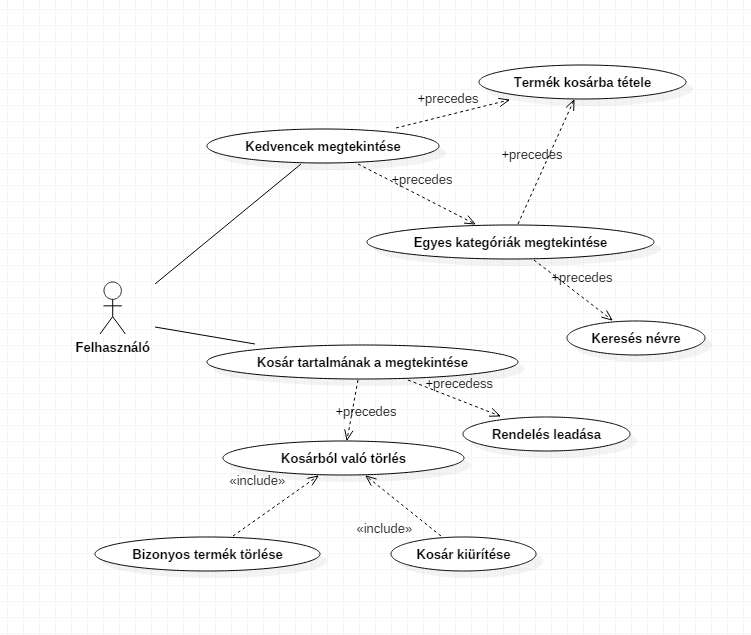
\includegraphics[scale=0.7]{usecase}
\subsection{Adminisztratív kliens}
\includegraphics[scale=0.7]{usecaseW}

\section{A rendszer szerkezete}
\subsection{Komponensek}
Az MVC acthitektúrának megfelelően a programnak 4 fontos komponense van.
\begin{itemize}
\item Az adatbázis felelős a rendszer által használt adatok, és a bevárlás lebonyolításához történő információk tárolására. Az adatbázishoz való kapcsolódást az  Entity Freamwork segítségével biztosítjuk.
\item A webes alkalmazási felület ASP.NET-ben MVC architektúrával megvalósítva, amely tartalmaz felhasználói nézeteket és ehhez kapcsolódó nézetmodelleket, kontrollereket, valamint az adatbázis modelljét, és a funkcionalitásért felelős kiszolgáló osztályokat.
\item Az adminisztratív grafikus alkalmazást WPF felhasználásával íródott , MVVM architektúrában.


\begin{center}
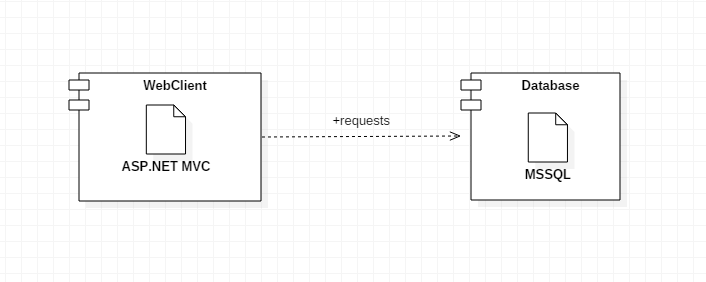
\includegraphics[scale=0.5]{component}
\end{center}

\end{itemize}
\subsection{Osztályok}

\subsubsection{Webes felhasználói felület}
\begin{itemize}
\item Külön project felelős az adatbázis modell megvalósításáért, mely kapcsolatban van az alkalmazást megvalósító modellel. 
\item A Models névtéren belül helyezkednek el a nézetmodellek,  valamint a bevásárlást végző osztályok.
\item A Controllers névtéren belül a kontrollerek helyezkednek el. A program 2 különböző kontrollere oszlik, valamint a közös funkcionalitást biztosító bázis kontrollere.
\item A View-en belül helyezkedik el a közös megjelenítésért felelős nézet, a kedvencek listázásáért felelős főoldali nézet,  a kosár tartalmát megjelenítő és a rendelés leadásáért felelős nézetek, valamint az egyek kategórákhoz tartozó ételek/italokrészleteit megadó felület
\end{itemize}

\begin{center}
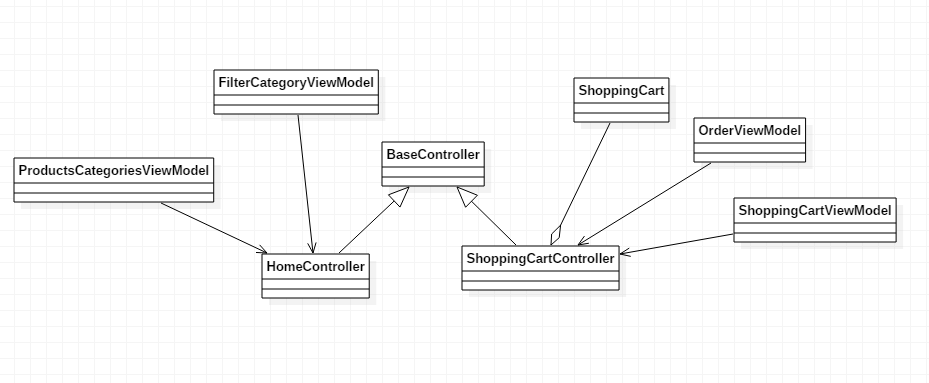
\includegraphics[scale=0.4]{classdiagram}
\end{center}

\subsubsection{Adminisztratív kliens}
\begin{itemize}
\item Az \textit{Admin} project felelős az alkalmazás megvalósításáért.
\item A grafikus konézetért a View névtérben lévő nézetek felelnek, ezeknek a dinamikus kinézete a ViewModel-hez tartozó osztályokhoz van kötve.
\item A funkciók megvalósításáért a Model névtér felelős, mely közvetlenül hívja a Persistence réteget, mely az adatbázissal kommunikál.  
\item Mivel az adatok JSON formátumban utaznak a szerves és az applikáció között így ezek konvertálásáért a DTO osztályok felelnek.
\end{itemize}

\begin{center}
\includegraphics[scale=0.5]{webapicomp}
\end{center}

Az egyes komponensek felépítése:
\begin{itemize}
\item ViewModel:

\begin{center}
\includegraphics[scale=0.5]{viewmodel}
\end{center}

\item Model:

\begin{center}
\includegraphics[scale=0.5]{model}
\end{center}

\item Persistence:

\begin{center}
\includegraphics[scale=0.5]{persistence}
\end{center}

\end{itemize}

\section{Adatbázis felépítése}
\begin{itemize}
\item Az adatbázisban tároljuk az egyes ételeket/italokat.
\item A különböző kategóriákat
\item Az adott felhasználó által leadott rendeléseket
\item A bevásárlás lebonyolításához szükséges adatokat
\end{itemize}
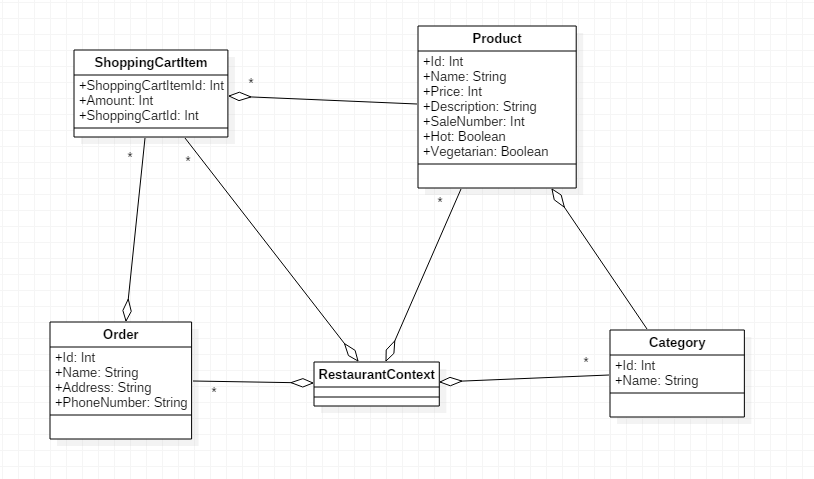
\includegraphics[scale=0.5]{database}

\end{document}